\documentclass[runningheads]{llncs}
\usepackage[review,year=2026,ID=11]{accv}
\usepackage{accvabbrv}
\usepackage{booktabs}
\usepackage{multirow}
\usepackage{graphicx}
\usepackage{amsmath}
\usepackage[pagebackref,breaklinks,colorlinks,citecolor=accvblue]{hyperref}
\hypersetup{pdftitle={Supplementary Material: Supervising Both Views: Camera Robustness under Label Scarcity}}
\usepackage[capitalize,noabbrev]{cleveref}
\setlength{\emergencystretch}{1em}
\newcommand{\miouc}{mIoU-C}

\begin{document}
\title{Supplementary Material:\\Supervising Both Views: Camera Robustness under Label Scarcity}
\author{Anonymous ACCV Workshop Submission}
\institute{Anonymous Institution}
\maketitle

\section{Reproducibility Details}

All experiments ran with PyTorch 2.13.0 and CUDA 13.0 on a single GPU with
24 GB of memory. Automatic mixed precision used
bfloat16 for model operations; losses and metrics were accumulated in float32
or float64. Random seeds initialize Python, NumPy, PyTorch, CUDA, the replacement
sampler, and deterministic corruption generators. Each configuration records the exact
labeled indices, class weights, package version, device name, training history,
validation scores, full confusion matrices, and every test condition in JSON.

Optimization uses AdamW with learning rate $3\times10^{-4}$, weight decay
$10^{-4}$, polynomial decay with power 0.9, and gradient clipping at norm 5,
validating every 100 updates. Every method receives the same sampled batches,
update count, pretrained initialization, checkpoint rule, and class weights.
ECE uses 15 equal-width confidence bins. Table values are rounded to one
decimal while deltas quoted in the main text are computed from full-precision
records, so the two can differ by 0.1.

Each budget resamples its labeled subset with replacement over the 400 updates.
The subsets are nested, so the 64-frame budget contains the 32-frame budget,
which contains the 16-frame budget. Only label-preserving corruptions are used:
every transformation alters pixel values but leaves geometry untouched, so the
mask stays valid for the corrupted view. Geometric corruptions such as
rolling-shutter skew would require warping the label and are outside this
protocol. Paired supervision and the two consistency variants compute two
forward passes per update, against one for ERM, ColorJitter, and CameraAug; we
hold the number of updates fixed rather than the compute, so part of their
advantage may follow from the larger effective batch.

The dataset loader reads the standard CamVid train/validation/test folders from
the public SegNet tutorial. RGB images and integer masks are resized to
$288\times384$ using bilinear and nearest-neighbor interpolation, respectively.
Class 11 is ignored. Inverse-square-root class weights are calculated only from
the chosen labeled subset, normalized to mean one, and clipped to $[0.35,3]$.

\section{Corruption Definitions}

Training samples one spatially aligned transform per batch: continuous
exposure/gamma change, channel-wise red/blue gain for white balance, additive
Gaussian noise, or Gaussian defocus blur. Evaluation fixes three severities for
eight families. Brightness is multiplicative; darkness combines gamma and gain;
white balance adjusts opposing red/blue gains; Gaussian and signal-dependent
shot noise model sensor degradation; defocus uses isotropic Gaussian kernels;
motion blur uses horizontal or vertical box kernels; and JPEG performs real
libjpeg encoding and decoding with severity-dependent quality and chroma
subsampling. Evaluation noise is seeded by condition and subset seed.

\section{Boundary Metric}

A semantic transition occurs wherever horizontally or vertically adjacent
valid pixels have different labels. For boundary F1, predicted and target
transition maps receive a two-pixel matching tolerance through max pooling.
Precision is the fraction of predicted boundary pixels within the target
neighborhood; recall is defined symmetrically. This class-agnostic transition
metric rewards localization but can count a nearby boundary of the wrong class
as a match, so per-class IoU remains the primary semantic metric.

\section{Complete Results and Qualitative Examples}

The code release contains aggregate CSV summaries, every per-run JSON record,
and the fixed split indices.

\Cref{tab:main-full} extends the main-paper table with the two aggregate
columns omitted there: the worst single corruption-family mIoU and 15-bin
expected calibration error under corruption.

\IfFileExists{../results/aggregate/table_main_full.tex}{
\begin{table*}[t]
\centering
\caption{Complete aggregate CamVid results. Values are mean $\pm$ 95\% $t$-interval over three nested-subset seeds. Worst is the lowest corruption-family mIoU; ECE is 15-bin expected calibration error under corruption (lower is better).}
\label{tab:main-full}
\small
\resizebox{\linewidth}{!}{%
\begin{tabular}{clrrrrrr}
\toprule
Labels & Method & Clean & \miouc{} & Held-out & Worst & Boundary F1 & ECE \\
\midrule
\multirow{6}{*}{16} & ERM & 37.5 $\pm$ 4.5 & 33.6 $\pm$ 2.4 & 32.2 $\pm$ 1.0 & 27.2 & 27.2 & 6.2 \\
 & ColorJitter & 37.7 $\pm$ 4.8 & 33.6 $\pm$ 4.0 & 32.1 $\pm$ 3.0 & 27.6 & 27.8 & 6.3 \\
 & CameraAug & 37.9 $\pm$ 3.3 & 34.1 $\pm$ 5.5 & 33.6 $\pm$ 5.9 & 29.0 & 29.9 & 6.7 \\
 & Paired CameraAug & 38.1 $\pm$ 4.2 & 34.9 $\pm$ 3.6 & 34.1 $\pm$ 3.3 & 31.7 & 29.9 & 6.7 \\
 & Uniform consistency & 38.4 $\pm$ 3.6 & 34.9 $\pm$ 3.7 & 34.1 $\pm$ 3.7 & 31.6 & 29.5 & 6.5 \\
 & BaCC & 38.1 $\pm$ 3.7 & 34.7 $\pm$ 2.1 & 34.1 $\pm$ 2.8 & 30.4 & 29.6 & 6.2 \\
\midrule
\multirow{6}{*}{32} & ERM & 41.7 $\pm$ 1.2 & 37.3 $\pm$ 2.3 & 35.5 $\pm$ 3.0 & 30.9 & 29.5 & 3.4 \\
 & ColorJitter & 41.8 $\pm$ 3.8 & 37.3 $\pm$ 3.7 & 35.6 $\pm$ 4.5 & 31.2 & 30.6 & 4.6 \\
 & CameraAug & 41.8 $\pm$ 0.5 & 37.7 $\pm$ 1.8 & 37.2 $\pm$ 1.6 & 32.9 & 32.0 & 4.9 \\
 & Paired CameraAug & 42.9 $\pm$ 1.1 & 38.8 $\pm$ 0.5 & 37.9 $\pm$ 1.2 & 34.8 & 32.3 & 4.0 \\
 & Uniform consistency & 42.6 $\pm$ 1.5 & 38.7 $\pm$ 1.0 & 37.9 $\pm$ 1.4 & 34.6 & 32.0 & 4.1 \\
 & BaCC & 42.8 $\pm$ 1.8 & 38.7 $\pm$ 1.8 & 37.9 $\pm$ 2.0 & 35.1 & 32.7 & 4.5 \\
\midrule
\multirow{6}{*}{64} & ERM & 46.4 $\pm$ 3.4 & 41.0 $\pm$ 2.9 & 38.7 $\pm$ 3.1 & 32.9 & 32.6 & 3.1 \\
 & ColorJitter & 46.1 $\pm$ 5.2 & 41.0 $\pm$ 3.6 & 38.8 $\pm$ 3.5 & 34.0 & 32.5 & 3.1 \\
 & CameraAug & 46.8 $\pm$ 1.6 & 42.1 $\pm$ 3.2 & 41.6 $\pm$ 3.3 & 35.6 & 34.4 & 2.4 \\
 & Paired CameraAug & 46.5 $\pm$ 2.8 & 42.1 $\pm$ 2.8 & 41.0 $\pm$ 2.6 & 37.9 & 34.6 & 3.2 \\
 & Uniform consistency & 46.7 $\pm$ 2.6 & 42.4 $\pm$ 2.6 & 41.4 $\pm$ 2.4 & 38.3 & 34.4 & 2.8 \\
 & BaCC & 46.6 $\pm$ 2.4 & 42.4 $\pm$ 2.4 & 41.4 $\pm$ 2.3 & 38.2 & 34.4 & 2.8 \\
\bottomrule
\end{tabular}}
\end{table*}

}{}

\Cref{tab:sequences} breaks clean test mIoU down by source video sequence at
32 labels. BaCC leads in both sequences, while CameraAug falls behind
ERM on Seq05VD.

\IfFileExists{../results/aggregate/table_sequences.tex}{
\begin{table}[t]
\centering
\caption{Clean test mIoU by source video sequence at 32 labels. Mean over three seeds.}
\label{tab:sequences}
\small
\begin{tabular}{lrr}
\toprule
Method & 0001TP & Seq05VD \\
\midrule
ERM & 40.7 & 40.8 \\
CameraAug & 42.4 & 40.4 \\
Uniform consistency & 42.1 & 41.2 \\
BaCC & 42.9 & 41.2 \\
\bottomrule
\end{tabular}
\end{table}

}{}

\Cref{tab:corruptions} breaks the aggregate \miouc{} down by corruption
family.

\IfFileExists{../results/aggregate/table_corruptions.tex}{
\begin{table*}[t]
\centering
\caption{Per-corruption mIoU at 32 labels, averaged over three severities and three seeds. Shot noise, motion blur, and JPEG are absent from training.}
\label{tab:corruptions}
\scriptsize
\setlength{\tabcolsep}{2.5pt}
\begin{tabular}{lrrrrrrrr}
\toprule
Method & Bright. & Dark & Defocus & Gauss. & JPEG & Motion & Shot & W. bal. \\
\midrule
ERM & 41.1 & 38.0 & 38.0 & 34.0 & 38.6 & 37.0 & 30.9 & 41.1 \\ 
CameraAug & 41.5 & 33.0 & 37.4 & 37.0 & 39.0 & 37.2 & 35.3 & 41.4 \\ 
Uniform & 42.1 & 35.6 & 38.6 & 37.2 & 39.8 & 38.5 & 35.3 & 42.1 \\ 
BaCC & 42.2 & 35.9 & 38.5 & 37.2 & 40.0 & 38.5 & 35.1 & 42.2 \\ 
\bottomrule
\end{tabular}
\end{table*}

}{}

\Cref{tab:ablation} sweeps the boundary weight $\alpha$ referenced in the main
paper's ablation discussion.

\IfFileExists{../results/aggregate/table_ablation.tex}{
\begin{table}[t]
\centering
\caption{Boundary-weight ablation and architecture check at 32 labels. Mean over three seeds.}
\label{tab:ablation}
\small
\begin{tabular}{llrrr}
\toprule Architecture & Setting & Clean & \miouc{} & Boundary F1 \\
\midrule
DeepLabV3 & $\alpha=0$ (uniform) & 42.6 & 38.7 & 32.0 \\
DeepLabV3 & $\alpha=1$ & 42.5 & 38.6 & 32.3 \\
DeepLabV3 & $\alpha=3$ & 42.8 & 38.7 & 32.7 \\
DeepLabV3 & $\alpha=6$ & 42.7 & 38.9 & 32.2 \\
\midrule
LR-ASPP & ERM & 44.3 & 36.1 & 42.1 \\
LR-ASPP & BaCC & 44.8 & 38.6 & 43.3 \\
\bottomrule
\end{tabular}
\end{table}

}{}

\Cref{tab:obstacle-classes} reports per-class IoU for the road-scene obstacle
categories most relevant to safety (pedestrians, bicyclists, signs, and cars).

\IfFileExists{../results/aggregate/table_obstacle_classes.tex}{
\begin{table}[t]
\centering
\caption{Corruption-averaged IoU for thin and obstacle-relevant classes at 32 labels (24 conditions, three seeds).}
\label{tab:obstacle-classes}
\small
\begin{tabular}{lrrrrr}
\toprule Method & Pole & Sign & Car & Ped. & Bike \\
\midrule
ERM & 4.5 & 3.8 & 49.7 & 11.3 & 4.6 \\
Paired & 6.2 & 7.9 & 50.8 & 13.8 & 5.0 \\
Uniform & 5.7 & 7.9 & 51.4 & 13.6 & 5.3 \\
BaCC & 6.2 & 7.8 & 51.8 & 13.2 & 5.6 \\
\bottomrule
\end{tabular}
\end{table}

}{}

Thin and rare classes remain difficult: even the best 32-label result is below
14 IoU for pedestrians and below 8 for signs. Paired camera supervision still more than
doubles sign IoU over ERM (7.9 versus 3.8) and lifts pedestrian IoU from 11.3
to 13.8. BaCC gives the highest car and bicyclist averages, while Paired
leads on pedestrians and signs.

\IfFileExists{../results/aggregate/qualitative.pdf}{
\begin{figure}[t]
\centering
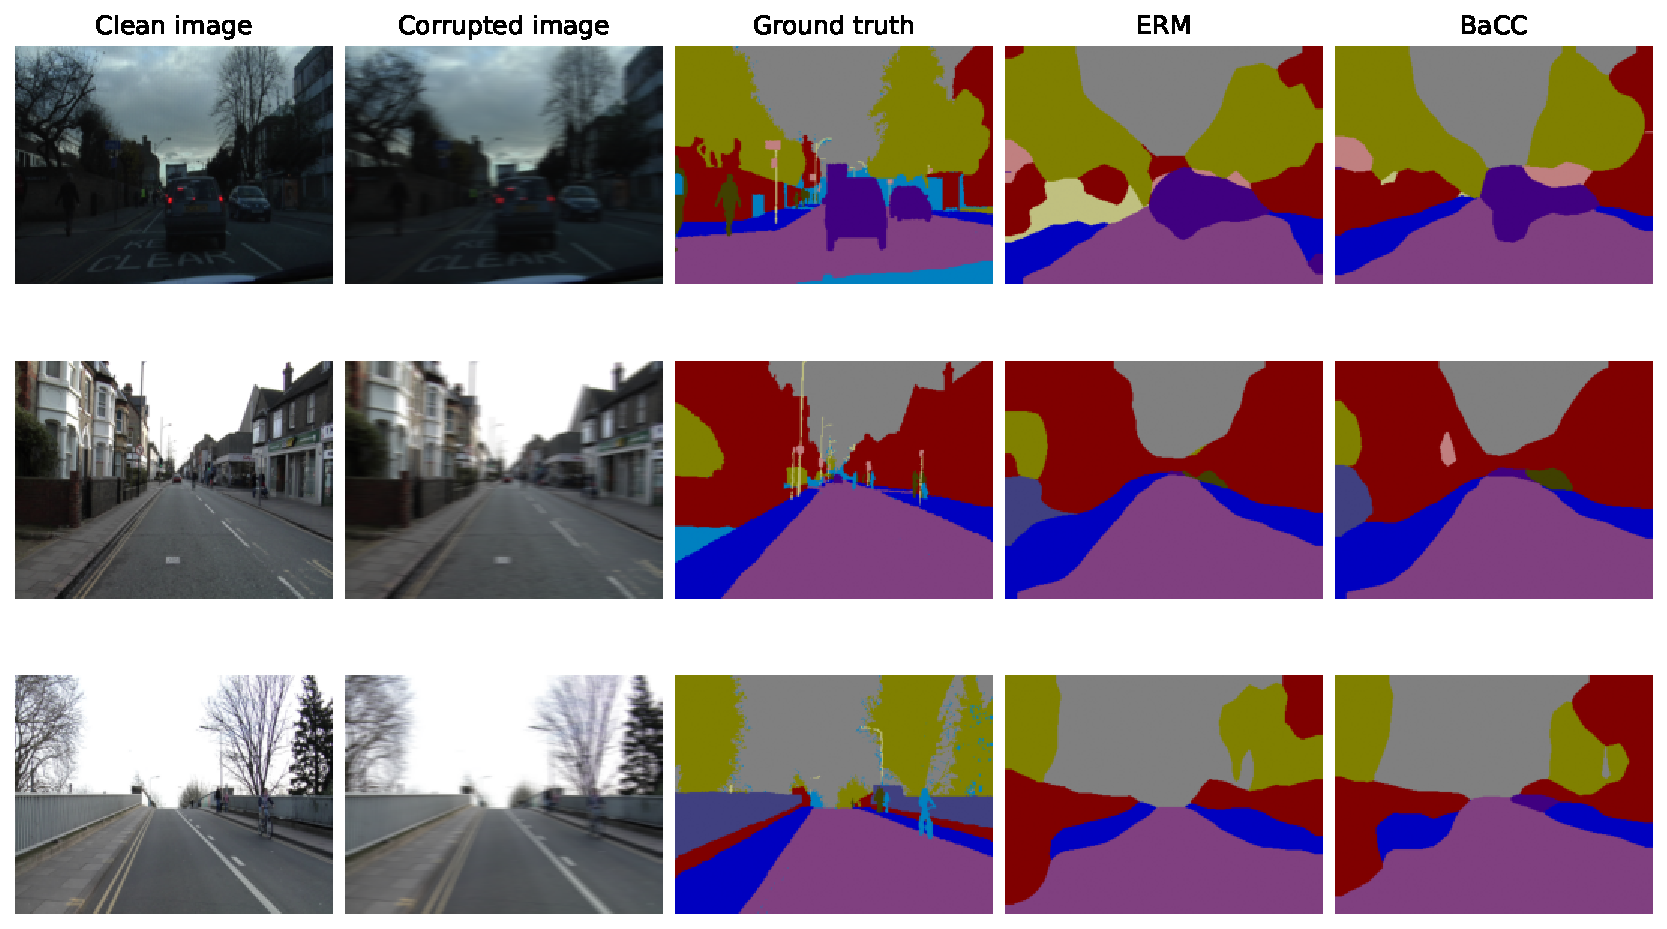
\includegraphics[width=\linewidth]{../results/aggregate/qualitative.pdf}
\caption{Representative held-out motion-blur examples at severity 3. Images
were selected by fixed test indices before viewing predictions.}
\end{figure}
}{Qualitative figures are generated by `python -m camrobust.visualize` from the
saved representative ERM and BaCC checkpoints.}

\section{Compute Cost}

The main grid uses a compact MobileNetV3 backbone and 400 updates per run. The 66 records sum to 1.12
run-hours; executing three interleaved shards took approximately 0.37 hours of
wall time on the single GPU. GPU identity and per-run time are stored in every
record. These measurements exclude setup, pilot experiments, and the two
checkpoint reruns used only for qualitative visualization.

\end{document}
